\documentclass[a4paper]{ctexart}
\usepackage{amsmath}
\usepackage[margin=2cm]{geometry} \pagestyle{plain}
\usepackage{tkz-euclide}
\renewcommand\parallel{\mathrel{/\mskip-2.5mu/}}
\begin{document}
    \begin{center}
        \textbf{\huge{第一节\qquad 相似三角形}} \vspace{5mm}
    \end{center}

    \begin{enumerate}
        \item 如图所示,在$\triangle ABC$中,$P$为$AB$上一点,$M$为$CP$的中点,$AC=2$,且满足$\angle PBM=\angle ACP$。若$AB=3$,求$BP$。\\
            \begin{flushright}
                \begin{tikzpicture}
                    \tkzDefPoints{0/0/B,4.5/0/C,2.5/2.2/P}
                    \tkzDefMidPoint(C,P) \tkzGetPoint{M}
                    \tkzFindAngle(P,B,M) \tkzGetAngle{anglePBM}
                    \tkzDefPointBy[rotation = center C angle \anglePBM](P) \tkzGetPoint{N}
                    \tkzInterLL(B,P)(C,N)\tkzGetPoint{A}
                    \tkzDrawPolygon(A,B,C)
                    \tkzDrawSegments(B,M C,P)
                    \tkzLabelPoints[right](M)
                    \tkzAutoLabelPoints[center = M](A,B,C,P)
                    \tkzMarkAngles[mark=none,size=0.5cm](M,B,P A,C,P)
                \end{tikzpicture}
            \end{flushright}
            \vspace{1cm}
        \item 如图所示,在菱形$ABCD$中,$E$是$BC$上一点,$F$是$CD$上一点,$\angle AFE=\angle ADC=\alpha $,$AE\perp EF$,$EC=3FC$,求$\cos\alpha$。\\
            \begin{flushright}
                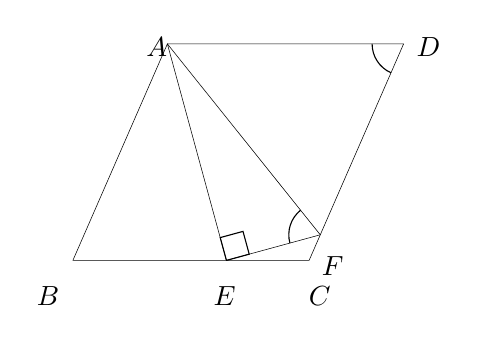
\begin{tikzpicture}
                    \tkzDefPoints{0/0/B,3/0/C}
                    \tkzDefPointBy[rotation = center B angle 66.42](C) \tkzGetPoint{A}
                    \tkzDefPointBy[translation = from B to C](A) \tkzGetPoint{D}
                    \tkzDefPointBy[homothety = center B ratio 0.65](C) \tkzGetPoint{E}
                    \tkzDefPointBy[rotation = center E angle -90](A) \tkzGetPoint{G}
                    \tkzDefMidPoint(A,C) \tkzGetPoint{H}
                    \tkzInterLL(E,G)(C,D) \tkzGetPoint{F}
                    \tkzDrawPolygon(A,B,C,D)
                    \tkzDrawSegments(A,E A,F E,F)
                    \tkzMarkAngles[mark=none,size=0.4cm](A,F,E A,D,C)
                    \tkzMarkRightAngle[size=0.3](A,E,F)
                    \tkzAutoLabelPoints[center = H](A,...,F)
                \end{tikzpicture}
            \end{flushright}
            \vspace{1cm}
        \item 如图所示,在等腰$\text{Rt}\triangle ABC$中,$\angle ACB=90^{\circ }$,$M$为$AB$上一点,$BE\perp CM$于点$E$,连接$AE$并延长交$BC$于点$F$。\\
        (1)若$EF$平分$\angle CEB$,求$\tan\angle CAF$。\\
        (2)在(1)的条件下,若$S_{\triangle CAE}=1$,求$AB$。\\
        \begin{flushright}
            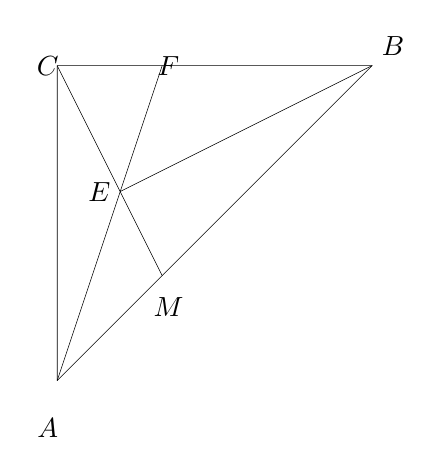
\begin{tikzpicture}
                \tkzDefPoints{0/0/A,0/4/C}
                \tkzDefPointBy[rotation = center C angle 90](A) \tkzGetPoint{B}
                \tkzDefPointBy[homothety = center A ratio 1/3](B) \tkzGetPoint{M}
                \tkzDefPointBy[projection = onto C--M](B) \tkzGetPoint{E}
                \tkzInterLL(A,E)(B,C) \tkzGetPoint{F}
                \tkzDrawPolygon(A,B,C)
                \tkzDrawSegments(A,F B,E C,M)           
                \tkzAutoLabelPoints[center =E](A,C,F,M)
                \tkzLabelPoints[left](E)
                \tkzLabelPoints[above right](B)
            \end{tikzpicture}
        \end{flushright}
        \vspace{1cm}
        \item 如图所示,等腰$\text{Rt}\triangle ABC$中,$BC=AC$,$E$为$AC$上一点,$D$为$AB$的中点,$DG\perp ED$交$AC$的延长线于点$G$,$FD$平分$\angle EDG$交$BC$的延长线于点$F$。\\ 
        (1)如图(a)所示,若$CE=2AE$,求$\dfrac{FD}{GD}$。\\ 
        (2)如图(b)所示,若$CE=nAE$($n>1$),求$\dfrac{FD}{GD}$。(用含有$n$的代数式表示)\\
        \begin{flushright}
            \begin{tabular}{cc}
                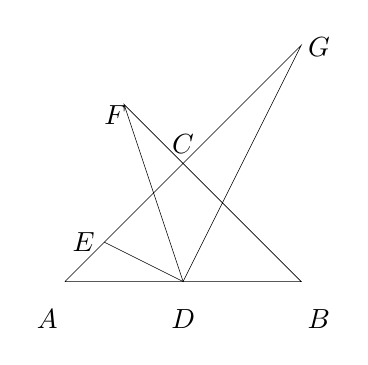
\begin{tikzpicture}
                    \tkzDefPoints{0/0/A,3/0/B,1.5/1.5/C}
                    \tkzDefPointBy[homothety = center A ratio 1/3](C) \tkzGetPoint{E}
                    \tkzDefMidPoint(A,B) \tkzGetPoint{D}
                    \tkzDefPointBy[rotation = center D angle -90](E) \tkzGetPoint{H}
                    \tkzInterLL(A,C)(D,H) \tkzGetPoint{G}
                    \tkzDefLine[bisector](E,D,G) \tkzGetPoint{I}
                    \tkzInterLL(D,I)(B,C) \tkzGetPoint{F}
                    \tkzDrawPolySeg(A,G,D,F,B,A)
                    \tkzDrawSegments(D,E)           
                    \tkzAutoLabelPoints[center =C](A,D,B,G,F)
                    \tkzLabelPoints[left](E)
                    \tkzLabelPoints[above](C)
                \end{tikzpicture}
                &
                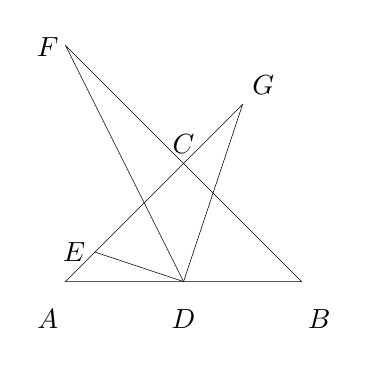
\begin{tikzpicture}
                    \tkzDefPoints{0/0/A,3/0/B,1.5/1.5/C}
                    \tkzDefPointBy[homothety = center A ratio 1/4](C) \tkzGetPoint{E}
                    \tkzDefMidPoint(A,B) \tkzGetPoint{D}
                    \tkzDefPointBy[rotation = center D angle -90](E) \tkzGetPoint{H}
                    \tkzInterLL(A,C)(D,H) \tkzGetPoint{G}
                    \tkzDefLine[bisector](E,D,G) \tkzGetPoint{I}
                    \tkzInterLL(D,I)(B,C) \tkzGetPoint{F}
                    \tkzDrawPolygon(A,G,D)
                    \tkzDrawPolygon(B,F,D)
                    \tkzDrawSegments(D,E)           
                    \tkzAutoLabelPoints[center =C](A,D,B,F)
                    \tkzLabelPoints[above](C)
                    \tkzLabelPoints[left](E)
                    \tkzLabelPoints[above right](G)
                \end{tikzpicture}\\ 
                (a)&(b)\\ 
            \end{tabular}
        \end{flushright}
        \vspace{3cm}
        \item 如图所示,已知矩形$ABCD$,点$E$、$F$、$P$分别在线段$AD$、$BC$、$DC$上,$BP$交$EF$于点$M$,$\angle EMP=45^{\circ }$,$AD=12$,$AB=6$,$BF=ED=4.5$,求$PC$。
        \begin{flushright}
            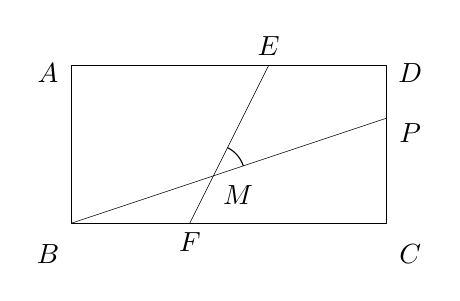
\begin{tikzpicture}
                \tkzDefPoints{0/0/B,4/0/C,0/2/A,4/2/D}
                \tkzDefPointBy[homothety = center B ratio 4.5/12](C) \tkzGetPoint{F}
                \tkzDefPointBy[homothety = center D ratio 4.5/12](A) \tkzGetPoint{E}
                \tkzDefPointBy[rotation = center F angle -45](E) \tkzGetPoint{G}
                \tkzDefLine[parallel=through B](F,G) \tkzGetPoint{H}
                \tkzInterLL(B,H)(C,D) \tkzGetPoint{P}
                \tkzInterLL(B,H)(E,F) \tkzGetPoint{M}
                \tkzDrawPolygon(A,B,C,D)
                \tkzDrawSegments(E,F B,P)
                \tkzDefMidPoint(A,C) \tkzGetPoint{O}          
                \tkzAutoLabelPoints[center =O](A,...,D,P)
                \tkzLabelPoints[below right](M)
                \tkzLabelPoints[below](F)
                \tkzLabelPoints[above](E)
                \tkzMarkAngles[mark=none,size=0.4cm](P,M,E)
            \end{tikzpicture}
        \end{flushright}
        \vspace{2cm}
        \item 如图所示,已知平行四边形$ABCD$中$\angle D=60^{\circ}$,点$E$、$F$分别在$AB$、$AD$上,$BF$交$CE$于点$M$。
        若$\triangle CFM$为等边三角形,$\cfrac{BC}{CD}=\cfrac{9}{8}$,求$\cfrac{BE}{CM}$。
        \begin{flushright}
            \begin{tikzpicture}
                \tkzDefPoints{0/0/B,3/0/C}
                \tkzDefPointBy[homothety = center B ratio 17/9](C) \tkzGetPoint{d}                
                \tkzDefPointBy[rotation = center C angle 60](d) \tkzGetPoint{D}
                \tkzDefPointBy[translation = from C to B](D) \tkzGetPoint{A}
                \tkzDefPointBy[rotation = center B angle 30](C) \tkzGetPoint{c}
                \tkzDefLine[mediator](B,C) \tkzGetPoints{e}{f}
                \tkzInterLL(e,f)(B,c) \tkzGetPoint{o}
                \tkzInterLC(A,D)(o,B) \tkzGetPoints{g}{F}
                \tkzDrawPolygon(A,B,C,D)
                \tkzDefPointBy[rotation = center C angle 60](F) \tkzGetPoint{M}
                \tkzInterLL(A,B)(C,M) \tkzGetPoint{E}
                \tkzDrawSegments(B,F F,C C,E)
                \tkzDefMidPoint(A,C) \tkzGetPoint{N}
                \tkzAutoLabelPoints[center =N](A,...,F)
                \tkzLabelPoints[below](M)
            \end{tikzpicture}
        \end{flushright}
        \vspace{2cm}
        \item 如图所示,在矩形$ABCD$中,$E$为$AD$的中点,将$\triangle ABE$沿$BE$折叠后得到$\triangle GBE$,点$G$在矩形$ABCD$的内部,延长$BG$交$DC$于点$F$。若$DF=CF$,求$\cfrac{AD}{AB}$。
        \begin{flushright}
            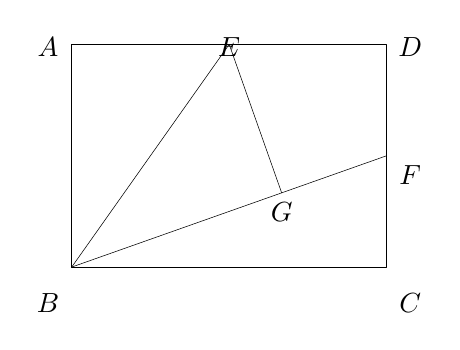
\begin{tikzpicture}
                \tkzDefPoints{0/0/B,4/0/C}
                \tkzDefPointBy[homothety = center B ratio 0.7071](C) \tkzGetPoint{a}                
                \tkzDefPointBy[rotation = center B angle 90](a) \tkzGetPoint{A}
                \tkzDefPointBy[translation = from B to C](A) \tkzGetPoint{D}
                \tkzDefMidPoint(A,D) \tkzGetPoint{E}
                \tkzDefMidPoint(D,C) \tkzGetPoint{F}
                \tkzInterLC(B,F)(B,A) \tkzGetPoints{g}{G}
                \tkzDrawPolygon(A,B,C,D)                
                \tkzDrawSegments(B,F B,E E,G)
                \tkzDefMidPoint(A,C) \tkzGetPoint{N}
                \tkzAutoLabelPoints[center =N](A,...,F)
                \tkzLabelPoints[below](G)
            \end{tikzpicture}
        \end{flushright}
        \vspace{2cm}
        \item 如图所示,在$\text{Rt}\triangle ABC$中,$E$为斜边的中点,点$D$在$AC$上,满足$\triangle AED=45^{\circ}$,
        将$\triangle ADE$沿$DE$翻折得到$\triangle FDE$,$EF$、$DF$分别交$BC$于点$M$、$N$。\\
        (1)如图(a)所示,若$\angle B=30^{\circ}$,求$\cfrac{MN}{AC}$。\\ 
        (2)如图(b)所示,若$AB=48$,$\cfrac{AC}{BC}=\cfrac{3}{4}$,求$MN$。
        \begin{flushright}
            \begin{tabular}{cc}
                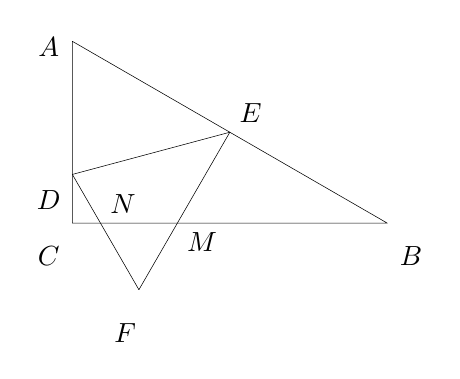
\begin{tikzpicture}
                    \tkzDefPoints{0/0/C,4/0/B}
                    \tkzDefLine[orthogonal = through C](C,B) \tkzGetPoint{a1}
                    \tkzDefPointBy[rotation = center B angle -30](C) \tkzGetPoint{a2}
                    \tkzInterLL(a1,C)(B,a2) \tkzGetPoint{A}
                    \tkzDefMidPoint(A,B) \tkzGetPoint{E}
                    \tkzDefPointBy[rotation = center E angle 45](A) \tkzGetPoint{a3}
                    \tkzDefPointBy[rotation = center E angle 45](a3) \tkzGetPoint{F}
                    \tkzInterLL(E,a3)(A,C) \tkzGetPoint{D}
                    \tkzInterLL(D,F)(B,C) \tkzGetPoint{N}
                    \tkzInterLL(E,F)(B,C) \tkzGetPoint{M}
                    \tkzDrawPolygon(A,B,C)
                    \tkzDrawSegments(D,E D,F E,F)           
                    \tkzAutoLabelPoints[center =E](A,D,C,F,B)
                    \tkzLabelPoints[below right](M)
                    \tkzLabelPoints[above right](N,E)
                \end{tikzpicture}
                &
                \begin{tikzpicture}
                    \tkzDefPoints{0/0/C,4/0/B,0/3/A}
                    \tkzDefMidPoint(A,B) \tkzGetPoint{E}
                    \tkzDefPointBy[rotation = center E angle 45](A) \tkzGetPoint{a3}
                    \tkzDefPointBy[rotation = center E angle 45](a3) \tkzGetPoint{F}
                    \tkzInterLL(E,a3)(A,C) \tkzGetPoint{D}
                    \tkzInterLL(D,F)(B,C) \tkzGetPoint{N}
                    \tkzInterLL(E,F)(B,C) \tkzGetPoint{M}
                    \tkzDrawPolygon(A,B,C)
                    \tkzDrawSegments(D,E D,F E,F)           
                    \tkzAutoLabelPoints[center =E](A,D,C,F,B)
                    \tkzLabelPoints[below right](M)
                    \tkzLabelPoints[above right](N,E)
                \end{tikzpicture}\\ 
                (a)&(b)\\ 
            \end{tabular}
        \end{flushright}
        \vspace{8cm}
        \item 如图所示,在矩形$ABCD$中,将$\triangle ABD$沿对角线$BD$翻折,得到$\triangle EBD$,连接$AE$交$BD$于点$G$,$DE$交$BC$于点$F$。\\ 
        (1)如图(a)所示,若$\cfrac{DC}{FC}=\cfrac{3}{4}$,求$\cfrac{AE}{BD}$。\\ 
        (2)如图(b)所示,若$\cfrac{AE}{BD}=\cfrac{24}{25}$,求$\cfrac{AB}{BC}$。\\
        \begin{flushright}
            \begin{tabular}{cc}
                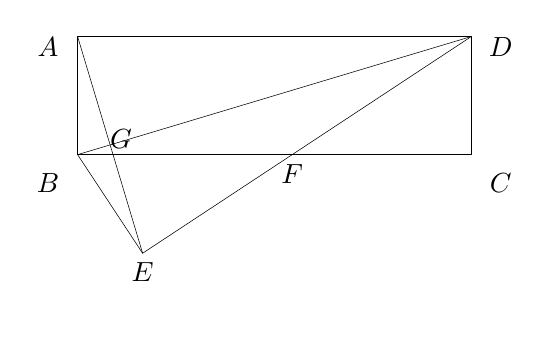
\begin{tikzpicture}
                    \tkzDefPoints{0/1.5/A,0/0/B,5/0/C,5/1.5/D}
                    \tkzDefPointBy[reflection = over B--D](A) \tkzGetPoint{E}
                    \tkzInterLL(A,E)(B,D) \tkzGetPoint{G}
                    \tkzInterLL(D,E)(B,C) \tkzGetPoint{F}
                    \tkzDrawPolygon(A,B,C,D)
                    \tkzDrawSegments(B,E D,E A,E B,D)
                    \tkzDefMidPoint(B,D) \tkzGetPoint{o}           
                    \tkzAutoLabelPoints[center = o](A,D,C,B)
                    \tkzDefPoint(-0.5,-2){n}
                    \tkzAutoLabelPoints[center = n](G)
                    \tkzLabelPoints[below](E,F)
                \end{tikzpicture}
                &\qquad
                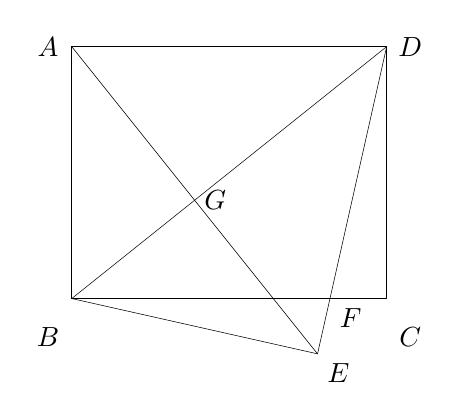
\begin{tikzpicture}
                    \tkzDefPoints{0/3.2/A,0/0/B,4/0/C,4/3.2/D}
                    \tkzDefPointBy[reflection = over B--D](A) \tkzGetPoint{E}
                    \tkzInterLL(A,E)(B,D) \tkzGetPoint{G}
                    \tkzInterLL(D,E)(B,C) \tkzGetPoint{F}
                    \tkzDrawPolygon(A,B,C,D)
                    \tkzDrawSegments(B,E D,E A,E B,D)
                    \tkzDefMidPoint(B,D) \tkzGetPoint{o}           
                    \tkzAutoLabelPoints[center = o](A,D,C,B)
                    %\tkzDefPoint(-0.5,-2){n}
                    \tkzLabelPoints[right](G)
                    \tkzLabelPoints[below right](E,F)
                \end{tikzpicture}\\ 
                (a)&(b)\\ 
            \end{tabular}
        \end{flushright}
        \vspace{7cm}
        \item 如图所示,在平面直角坐标系$xOy$中,矩形$AOCB$截反比例函数$y=\cfrac{k}{x}$($k>0$,$x>0$)的图像于点
        $E$、$F$,将$\triangle BEF$沿$EF$翻折,点$B$恰好落在$x$轴正半轴的点$D$处。已知$AB=2A0=4$,求$k$。\\
        \begin{flushright}
            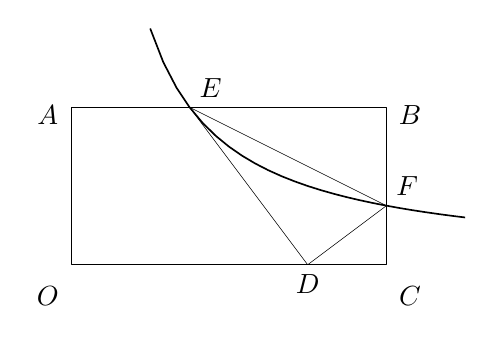
\begin{tikzpicture}[domain = 1:5,line width=0.6pt]
                \tkzInit[xmax=5.5,ymax=3.5]
                \tkzDrawXY[noticks,>=latex]
                \tkzDefPoints{0/0/O,0/2/A,4/2/B,4/0/C,3/0/D}
                \tkzDefLine[mediator](B,D) \tkzGetPoints{e}{f}
                \tkzInterLL(e,f)(B,A) \tkzGetPoint{E}
                \tkzInterLL(e,f)(B,C) \tkzGetPoint{F}
                \tkzGetPointCoord(E){g}
                \draw plot (\x,{(\gx)*(\gy)/(\x)});
                \tkzDrawPolygon(A,B,C,O)                
                \tkzDrawPolygon(E,F,D)
                \tkzDefMidPoint(A,C) \tkzGetPoint{N}
                \tkzAutoLabelPoints[center = N](A,B,C,O)
                \tkzLabelPoints[below](D)
                \tkzLabelPoints[above right](E)
                \tkzLabelPoints[above right](F)
            \end{tikzpicture}
        \end{flushright}
        \vspace{2cm}
        \item 如图所示,在矩形$ABCD$中,$E$为$BC$上一点,将$\triangle ABE$沿$AE$翻折得到$\triangle AFE$,且点$F$在
        对角线$AC$下方,连接$CF$,恰有$CF=DC$,作$FH\perp BC$于点$H$。已知$AB= 4\sqrt{5}$,$BC=4\sqrt{11}$,求$FH$。
        \begin{flushright}
            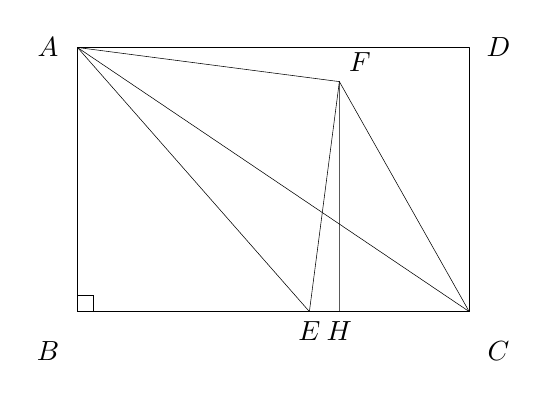
\begin{tikzpicture}
                \tkzDefPoint(0,0){B}
                \tkzDefPoint(0,{1.5*sqrt(5)}){A}
                \tkzDefPoint({1.5*sqrt(11)},0){C}
                \tkzDefPoint({1.5*sqrt(11)},{1.5*sqrt(5)}){D}
                \tkzDefLine[mediator](A,C) \tkzGetPoints{a}{c}
                \tkzInterLC(a,c)(C,D) \tkzGetPoints{F}{k}
                \tkzDefMidPoint(B,F) \tkzGetPoint{e}
                \tkzDefMidPoint(A,C) \tkzGetPoint{c}
                \tkzInterLL(A,e)(B,C) \tkzGetPoint{E}
                \tkzDefPointBy[projection = onto B--C](F) \tkzGetPoint{H}
                \tkzDrawPolygon(A,B,C,D)
                \tkzDrawSegments(A,C A,E A,F E,F F,H F,C)
                \tkzAutoLabelPoints[center = c](A,B,C,D)
                \tkzLabelPoints[below](E,H)
                \tkzLabelPoints[above right](F)
                \tkzMarkRightAngle[size=0.2](A,B,C)
            \end{tikzpicture}
        \end{flushright}
        \vspace{1.5cm}
        \item 如图所示,在正方形$ABCD$中,$E$为$BC$上一点,将$\triangle DCE$沿$DE$翻折得到$\triangle DFE$。
        若$DF$、$DE$恰好与以正方形$ABCD$的中心为圆心的$\odot O$相切,连接$FO$,求$\cfrac{FO}{DE}$。\\
        \begin{flushright}
            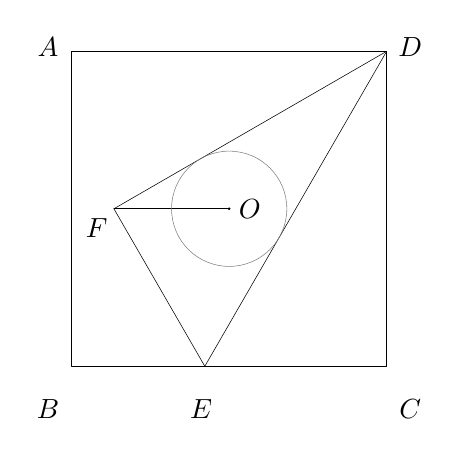
\begin{tikzpicture}
                \tkzDefPoints{0/0/B,4/0/C}
                \tkzDefSquare(B,C) \tkzGetPoints{D}{A}
                \tkzDefPointBy[rotation = center D angle -60](C) \tkzGetPoint{F}
                \tkzDefLine[bisector](F,D,C) \tkzGetPoint{e}
                \tkzInterLL(D,e)(B,C) \tkzGetPoint{E}
                \tkzDefMidPoint(A,C) \tkzGetPoint{O}
                \tkzDefPointBy[projection = onto D--E](O) \tkzGetPoint{o}
                \tkzDrawPolygon(A,B,C,D)
                \tkzDrawSegments(D,F D,E E,F O,F)
                \tkzDrawCircle(O,o)
                \tkzAutoLabelPoints[center = O](A,...,F)
                \tkzDrawPoint[size=0.5](O)
                \tkzLabelPoints[right](O)
            \end{tikzpicture}
        \end{flushright}
        \vspace{1.5cm}
        \item 如图所示,在矩形$ABCD$中,$AB=10$,$BC=14$,$P$为$AB$上一点,将$\triangle PBC$沿$PC$翻折得到
        $\triangle PEC$,$PE$交$AD$于点$F$,$CE$交$AD$于点$G$。若$AF=4$,求$GD$。\\
        \begin{flushright}
            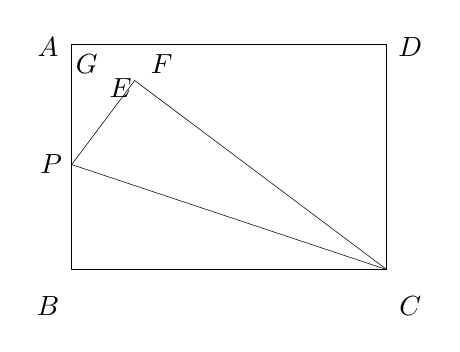
\begin{tikzpicture}
                \tkzDefPoints{0/0/B,4/0/C}
                \tkzDefPoint(0,{4/1.4}){A}
                \tkzDefPoint(4,{4/1.4}){D}
                \tkzDefPointBy[homothety = center A ratio 2/7](D) \tkzGetPoint{F}
                \tkzInterLC(A,B)(C,F) \tkzGetPoints{p}{q}
                \tkzDefLine[bisector](F,C,q) \tkzGetPoint{e}
                \tkzInterLL(C,e)(A,B) \tkzGetPoint{P}
                \tkzDefPointBy[projection = onto P--F](C) \tkzGetPoint{E}
                \tkzInterLL(C,E)(A,D) \tkzGetPoint{G}
                \tkzDrawPolygon(A,B,C,D)
                \tkzDrawSegments(C,P P,E E,C)
                \tkzDefMidPoint(A,C) \tkzGetPoint{O}
                \tkzAutoLabelPoints[center = O](A,...,E)
                \tkzLabelPoints[below](F,G)
                \tkzLabelPoints[left](P)
            \end{tikzpicture}
        \end{flushright}
        \vspace{2cm}
        \item 如图所示,在正方形$ABCD$中,$AB=15$,点$E$在边$CD$上,连接$AE$,交对角线$BD$于点$Q$,将$\triangle ADE$
        沿$AE$翻折,点$D$落在点$F$处,$O$是对角线$BD$的中点,连接$OF$并延长与$CD$相交于点$G$。若$\cfrac{EF}{AB}=\cfrac{1}{3}$,求$FG$。
        \begin{flushright}
            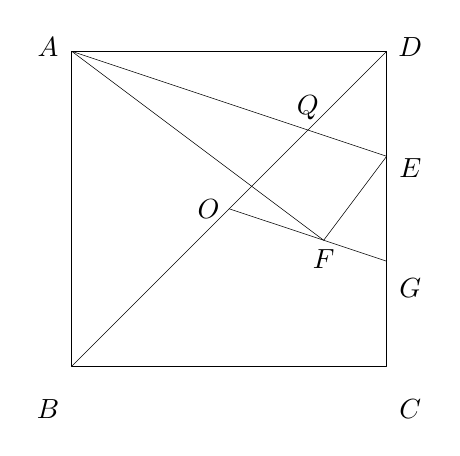
\begin{tikzpicture}
                \tkzDefPoints{0/0/B,4/0/C}
                \tkzDefSquare(B,C) \tkzGetPoints{D}{A}
                \tkzDefMidPoint(B,D) \tkzGetPoint{O}
                \tkzDefPointBy[homothety = center D ratio 1/3](C) \tkzGetPoint{E}
                \tkzDefPointBy[reflection = over A--E](D) \tkzGetPoint{F}
                \tkzInterLL(O,F)(C,D) \tkzGetPoint{G}
                \tkzInterLL(A,E)(B,D) \tkzGetPoint{Q}
                \tkzDrawPolygon(A,B,C,D)
                \tkzDrawSegments(A,E E,F F,A B,D O,G)
                \tkzAutoLabelPoints[center = O](A,...,E,G)
                \tkzLabelPoints[below](F)
                \tkzLabelPoints[left](O)
                \tkzLabelPoints[above](Q)
            \end{tikzpicture}
        \end{flushright}
        \vspace{1.5cm}
        \item 如图所示,在菱形$ABCD$中,$\tan A=\cfrac{4}{3}$,点$M$、$N$分别在边$AD$、$BC$上,将四边形$AMNB$沿
        $MN$翻折,使$AB$的对应线段$EF$经过顶点$D$,当$EF\perp AD$时,求$\cfrac{BN}{CN}$。
        \begin{flushright}
            \begin{tikzpicture}
                \tkzDefPoints{0/0/A,3.6/0/B}
                \tkzDefPoint(53.13:3.6){D}
                \tkzDefPointBy[translation = from A to D](B) \tkzGetPoint{C}
                \tkzDefPointBy[homothety = center D ratio 4/9](A) \tkzGetPoint{M}
                \tkzDefPointBy[reflection = over A--E](D) \tkzGetPoint{F}
                \tkzDefShiftPoint[M](90:2){E}
                \tkzDefLine[mediator](A,E) \tkzGetPoints{m}{n}
                \tkzInterLL(m,n)(B,C) \tkzGetPoint{N}
                \tkzDefLine[parallel = through N](M,E)  \tkzGetPoint{f}
                \tkzInterLL(N,f)(E,D) \tkzGetPoint{F}
                \tkzDrawPolygon(M,N,C,D)
                \tkzDrawPolygon(M,N,F,E)
                \tkzDrawSegments[dashed](A,M A,B B,N)
                \tkzMarkRightAngle(E,D,M)
                \tkzLabelPoints[right](B,C,N,F)
                \tkzLabelPoints[left](A,M,E)
                \tkzLabelPoints[above](D)
            \end{tikzpicture}
        \end{flushright}
        \vspace{1.5cm}
        \item 如图所示,在矩形$ABCD$中,$F$为$CD$上一点,将$\triangle ADF$沿$AF$翻折得到$\triangle AEF$,点$E$恰好
        落在$BC$上,作$EG \parallel CD$交$AF$于点$G$,连接$DG$。\\ 
        (1)求证:四边形$DGEF$为菱形。\\ 
        (2)若$AG=6$,$EG=2\sqrt{5}$,求$GF$。
        \begin{flushright}
            \begin{tikzpicture}
                \tkzDefPoints{0/0/B,4/0/C,0/3/A,4/3/D}
                \tkzInterLC(B,C)(A,D) \tkzGetPoints{E}{e}
                \tkzDefLine[bisector](E,A,D) \tkzGetPoint{f}
                \tkzInterLL(A,f)(C,D) \tkzGetPoint{F}
                \tkzDefLine[parallel = through E](C,D) \tkzGetPoint{g}
                \tkzInterLL(E,g)(A,F) \tkzGetPoint{G}
                \tkzDrawPolygon(A,B,C,D)
                \tkzDrawSegments(A,E A,F G,E G,D E,F)
                \tkzLabelPoints[right](C,D,F)
                \tkzLabelPoints[left](A,B)
                \tkzLabelPoints[above](G)
                \tkzLabelPoints[below](E)
            \end{tikzpicture}
        \end{flushright}
        \vspace{1.5cm}
    \end{enumerate}
\end{document}